\subsection{Physical Structure}
The structure of the robot should allow the movement of the robot across the map. 
That means, the robot should have at least two motors to move in the plane of the circuit and a minimum of two light sensors to check its position referred to the black lines of the map and check when the robot has arrived to a crossroad.

\subsubsection{Motor configuration and control}
The chosen motor configuration consist in the use of two motors that move two parallel wheels. 
This allows the robot to change the direction of the movement setting a different motor speed on each motor.

To follow the line, the robot should be able to turn, what means that the motors should be set to different speeds.
These speeds are chosen with a P controller.
This controller slows down the speed of one or another wheel in function of the perpendicular displacement of the sensors 
over the line. 


\subsubsection{Sensor configuration}

Three light sensors are used as seen in figure \ref{fig:robotscheme}. 
Two of these sensors are used in the line following control and are placed in the front of the robot.
The distance between them is of 40mm, which is bigger than te line width.
This gives to the controller a big actuation rank, as the distance between the sensors is bigger than the width of the line.

In the position control, the value of the sensors are compared and the robot is controlled having in mind that the value of the sensors should be the same when the robot is centred above the line.
When the value of both sensors are low, the robot is facing a crossroad.


About the third sensor, it is placed in the back of the robot, just before the wheels.
It is used to detect the lines of the crossroads when going back and turning.

This sensor is placed the closest possible to the wheel's axis, and far enough to the robot center so it is not affected
for the followed line.

About the light levels in the room, it has been tested and proved that the sensors are highly sensitive to changes in 
the ambient light levels, specially under sunlight exposure. 

The first solution chosen to solve this problem has been use a shield around the three sensors, so the ambient light 
doesn't affect the measures.
This has shown a good result working in the lab, and under sunlight in cloudy days, but was unable to work in sunny days,
as the sensors were still afected for the sunlight intensity.
To minimize the effect of the sun, a second shield has been placed covering the robot base, so the sensors are allways in
shadows.
This system has shown to be robust under all conditions.



\subsubsection{Tool configuration}

To be able to push and guide the can across the map, the robot should have a proper tool that allows this task. 
The proposed design consist of two bars placed making an angle that allows the guide of the bottle when driving straight forward, as is shown in figure \ref{fig:robotscheme}.
This configuration allows catching the can even when its position is displaced, making the robot's job more easy.

Considering the rules of the game then the can is not permitted to be pushed left or right and because of that, no special design enabling this are required.


The final build of the robot is seen in figure \ref{fig:robotImage}.

\begin{figure}[H]
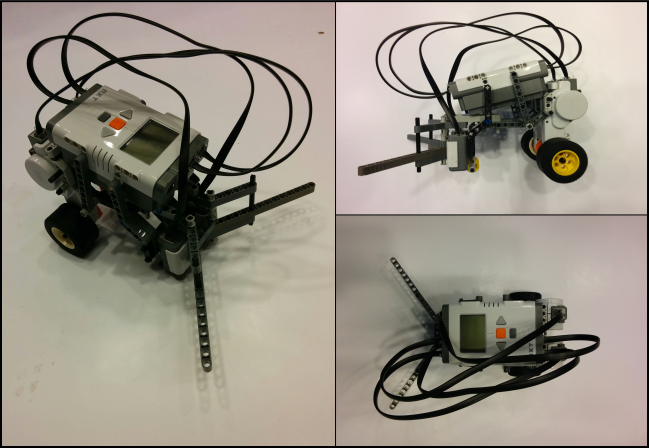
\includegraphics[width=10cm]{Fig1.png}
\centering
\caption{Images of the built robot.}
\label{fig:robotImage}
\end{figure}

